\section{Paradigma No 06 – PRINCIPIO DE DISEÑO SOLID} 



\begin{enumerate}[1.]


\item INTRODUCCION:


Solid es un acrónimo inventado por Robert C. Martin para establecer los cinco principios básicos de la programación orientada a objetos y diseño. Este acrónimo tiene bastante relación con los patrones de diseño, en especial, con la alta cohesión y el bajo acoplamiento.
El objetivo de tener un buen diseño de programación es abarcar la fase de mantenimiento de una manera más legible y sencilla, así como conseguir crear nuevas funcionalidades sin tener que modificar en gran medida código antiguo. 


El objetivo de tener un buen diseño de programación es abarcar la fase de mantenimiento de una manera más legible y sencilla, así como conseguir crear nuevas funcionalidades sin tener que modificar en gran medida código antiguo. 


\item Responsabilidad simple:

Este principio trata de destinar cada clase a una finalidad sencilla y concreta. En muchas ocasiones estamos tentados a poner un método reutilizable que no tienen nada que ver con la clase simplemente porque lo utiliza y nos pilla más a mano. En ese momento pensamos "Ya que estamos aquí, para que voy a crear una clase para realizar esto.

El problema surge cuando tenemos la necesidad de utilizar ese mismo método desde otra clase. Si no se refactoriza en ese momento y se crea una clase destinada para la finalidad del método, nos toparemos a largo plazo con que las clases realizan tareas que no deberían ser de su responsabilidad.

\item Abierto/Cerrado:

Es decir, el diseño debe ser abierto para poderse extender, pero cerrado para poderse modificar. Aunque dicho parece fácil, lo complicado es predecir por donde se debe extender y que no tengamos que modificarlo. Para conseguir este principio hay que tener muy claro cómo va a funcionar la aplicación, por donde se puede extender y cómo van a interactuar las clases.

El uso más común de extensión es mediante la herencia y la reimplementación de métodos. Existe otra alternativa que consiste en utilizar métodos que acepten una interface de manera que podemos ejecutar cualquier clase que implemente ese interface. En todos los casos, el comportamiento de la clase cambia sin que hayamos tenido que tocar código interno.


\item Sustitucion Liskov:

Este principio fue creado por Barbara Liskov y habla de la importancia de crear todas las clases derivadas para que también puedan ser tratadas como la propia clase base. Cuando creamos clases derivadas debemos asegurarnos de no Re implementar métodos que hagan que los métodos de la clase base no funcionases si se tratasen como un objeto de esa clase base.



\item SEGREGACION DEL INTERFACE:

Este principio fue formulado por Robert C. Martin y trata de algo parecido al primer principio. Cuando se definen interfaces estos deben ser específicos a una finalidad concreta. Por ello, si tenemos que definir una serie de métodos abstractos que debe utilizar una clase a través de interfaces, es preferible tener muchos interfaces que definan pocos métodos que tener un interface con muchos métodos.
El objetivo de este principio es principalmente poder reaprovechar los interfaces en otras clases. Si tenemos una interface que compara y clona en el misma interface, de manera más complicada se podrá utilizar en una clase que solo debe comparar o en otra que solo debe clonar.

\item INVERSIÓN DE DEPENDENCIAS:

También fue definido por Robert C. Martin. El objetivo de este principio conseguir desacoplar las clases. En todo diseño siempre debe existir un acoplamiento, pero hay que evitarlo en la medida de lo posible. Un sistema no acoplado no hace nada, pero un sistema altamente acoplado es muy difícil de mantener.
El objetivo de este principio es el uso de abstracciones para conseguir que una clase interactúe con otras clases sin que las conozca directamente. Es decir, las clases de nivel superior no deben conocer las clases de nivel inferior. Dicho de otro modo, no debe conocer los detalles. Existen diferentes patrones como la inyección de dependencias o servicie locator que nos permiten invertir el control.



	
\begin{center}
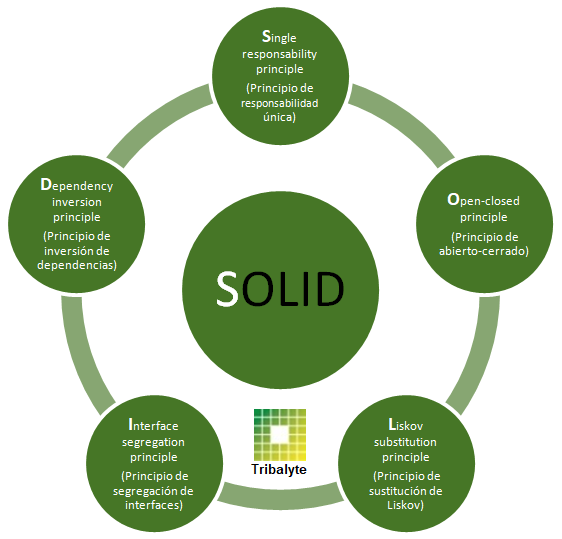
\includegraphics[scale=0.50]{./Imagenes/img12.png} 
\end{center}


\end{enumerate}